\documentclass[]{report}
\usepackage{amsmath,amsfonts}
\usepackage{graphicx}
\usepackage{float}
\usepackage{url}
\usepackage{tikz}
\usepackage{amsmath}
\usepackage{booktabs}
\setcounter{MaxMatrixCols}{13}
\usepackage[hidelinks,hypertexnames=false]{hyperref}
\usetikzlibrary{arrows.meta, decorations.pathreplacing, decorations.pathmorphing}

% Title Page
\title{{\huge  Longitudinal Active Suspension Control in a Half-Car Model with Unsprang Masses} \\
	{\small Automatic Control\\
		Electronic Engineering for Intelligent Vehicles\\
		University of Bologna\\
		A.A. 2025-2026}}
\author{Alessandro Briccoli, Cristian Cecchini, Mario Di Marino}


\begin{document}

	
	\maketitle
	
	\begin{abstract}
		This report presents the modeling, design, and simulation of an active suspension control system aimed at improving ride comfort and handling performance in passenger vehicles. The study focuses on a half-car model that includes both front and rear suspension dynamics, allowing the analysis of vertical and pitch motion of the vehicle body. Unlike passive suspension systems, which rely solely on spring-damper elements, the active suspension system introduced here incorporates actuators capable of generating controlled forces to counteract road disturbances in real time.
		
		To achieve the desired ride quality, a control strategy based on Proportional-Integral-Derivative (PID) controllers is developed.  Additionally, a state estimation technique using a Kalman observer is incorporated to provide real-time estimates of the states, helping to adapt to acceleration and road profile in a faster and more effective way.
		
		The performance of the control system is evaluated through simulations conducted in MATLAB/Simulink. Results show a significant reduction in body acceleration and pitch angle variation when compared to a passive suspension system, demonstrating the effectiveness of the proposed approach in enhancing ride comfort. This project perfectly demonstrates, once again, the massive importance of active control strategies in automotive suspension design.
	\end{abstract}
	
	\chapter{Introduction}
\section{Motivations}
Suspension systems play a crucial role in ensuring vehicle stability, comfort, and safety. Traditional passive suspensions cannot adapt to changing road conditions, leading to undesired oscillations and reduced performance. 

In this project, focus on active suspension control in the longitudinal direction (front and rear), which aims to reduce vertical oscillations and pitch movements when the vehicle passes over bumps or uneven surfaces. The goal is to design a control system that keeps the car body as steady as possible, improving both passenger comfort and vehicle handling.

The half-car model was chosen because it provides a good trade-off between model simplicity and dynamic realism and allows to study the impact of front and rear suspension forces on the vehicle behavior without dealing with the complexity of a full 3D model.

	
%	\section{Contributions}
%	Describe what this project deals with. What has been done to solve the problem presented in the motivations.
	
%	\section{State of art and literature comparison}
%	List the closest works that deal with the same problem and compare the achievement obtained and the strategies exploited in %   this paper. For the search of the literature use \url{https://ieeexplore.ieee.org/Xplore/home.jsp} and  %      %\url{https://www.sciencedirect.com/}.
	
%	\section{Organisation of the manuscript}
%	Describe what the reader finds in each of the Sections of this manuscript.
	



\section{List of the symbols}
\begin{table}[H]
	\centering
	\caption{Symbol Table}
	\begin{tabular}{lll}
		\toprule
		\textbf{Symbol} & \textbf{Description} & \textbf{Dimension} \\
		\midrule
		$x$ & State vector & $\mathbb{R}^{12}$ \\
		$u$ & Control input vector $[u_1\;u_2]^T$ & $\mathbb{R}^{2}$ \\
		$y$ & Measured output vector & $\mathbb{R}^{5}$ \\
		$e$ & Control error vector & $\mathbb{R}^{2}$ \\
		$d$ & Disturbance vector & $\mathbb{R}^{6}$ \\
		$r$ & Reference vector $[r_z\; r_\theta]^T$ & $\mathbb{R}^{2}$ \\
		$\nu$ & Sensor noise vector & $\mathbb{R}^{5}$ \\
		$w$ & Exogenous input $w=\mathrm{col}(d,\nu,r)$ & --- \\
		
		$p_z$ & Vertical displacement of vehicle CoM & m \\
		$v_z$ & Vertical velocity of vehicle CoM & m/s \\
		$\theta$ & Pitch angle of vehicle body & rad \\
		$\dot{\theta}$ & Pitch angular velocity & rad/s \\
		
		$h_{wf}, h_{wr}$ & Front and rear wheel vertical displacement & m \\
		$\dot{h}_{wf}, \dot{h}_{wr}$ & Front and rear wheel vertical velocity & m/s \\
		
		$\theta_{gf}, \theta_{gr}$ & Road pitch angle at front and rear axle & rad \\
		$z_{gf}, z_{gr}$ & Road vertical displacement at front and rear axle & m \\
		
		$u_1$ & Total vertical actuator force & N \\
		$u_2$ & Pitch moment component of actuator input & Nm \\
		$f_{af}, f_{ar}$ & Front and rear actuator forces & N \\
		
		$d_f, d_r$ & Distance from CoM to front and rear axle & m \\
		$h_{cg}$ & Height of vehicle center of mass & m \\
		
		$m$ & Sprung mass (vehicle body) & kg \\
		$m_{wf}, m_{wr}$ & Front and rear unsprung mass & kg \\
		$J$ & Pitch moment of inertia & kg\,m$^2$ \\
		
		$k_f, k_r$ & Front and rear suspension stiffness & N/m \\
		$\beta_f, \beta_r$ & Front and rear suspension damping & N\,s/m \\
		
		$k_{tf}, k_{tr}$ & Front and rear tire stiffness & N/m \\
		
		$s_1, s_3$ & Front and rear suspension deflection & m \\
		$s_2, s_4$ & Front and rear suspension velocity & m/s \\
		
		$f_{sf}, f_{sr}$ & Front and rear suspension forces & N \\
		$f_{wf}, f_{wr}$ & Front and rear wheel dynamics forces & N \\
		
		$f_{x f}, f_{x r}$ & Longitudinal forces at front and rear axle & N \\
		$F_x$ & Total longitudinal force $F_x=f_{xf}+f_{xr}$ & N \\
		
		$f_2$ & Vertical acceleration of vehicle body & m/s$^2$ \\
		$f_4$ & Pitch angular acceleration & rad/s$^2$ \\
		
		$\alpha_{gf}, \alpha_{gr}$ & Road pitch angular acceleration (front, rear) & rad/s$^2$ \\
		$\dot{z}_{gf}, \dot{z}_{gr}$ & Road vertical velocity (front, rear) & m/s \\
		
		$y_x$ & Longitudinal accelerometer output & m/s$^2$ \\
		$y_z$ & Vertical accelerometer output & m/s$^2$ \\
		$y_\theta$ & Gyroscope pitch-rate measurement & rad/s \\
		$y_f, y_r$ & Front and rear suspension sensors & m \\
		
		$\nu_y, \nu_z, \nu_g, \nu_f, \nu_r$ & Sensor noise components & --- \\
		
		$r_z$ & Reference vertical position & m \\
		$r_\theta$ & Reference pitch angle & rad \\
		
		$g$ & Gravitational acceleration & m/s$^2$ \\
		$\gamma_f$ & Anti-Dive suspension inclination & --- \\
		$\gamma_r$ & Anti-Squat suspension inclination & --- \\
		\bottomrule
	\end{tabular}
\end{table}



	
%	\chapter{Active Suspensions Control System}
%
%	
%	\section{Model and Problem Formulation}
%	In this section, the formulation of the control problem for the active suspension system of a half-car model. This system aims to regulate both the vertical position and the perceived pitch angle of the vehicle body, enhancing ride comfort and handling. The model is described by a nonlinear dynamic system influenced by road disturbances, actuator forces, and sensor measurements.
%	
%	The general form of the system is expressed as:
%	\begin{align}
%		\dot{x} &= f(x, u, w) \\
%		y &= h(x, u, w) \\
%		e &= h_e(x, u, w)
%	\end{align}
%	
%	Where:
%	\begin{itemize}
%		\item $x \in \mathbb{R}^n$ is the \textbf{state vector},
%		\item $u \in \mathbb{R}^p$ is the \textbf{control input vector},
%		\item $y \in \mathbb{R}^q$ is the \textbf{measured output vector},
%		\item $e \in \mathbb{R}^{l_m}$ is the \textbf{control error (goal)},
%		\item $d \in \mathbb{R}^{l_d}$ is the \textbf{disturbance vector},
%		\item $r \in \mathbb{R}^{l_r}$ is the \textbf{reference signal},
%		\item $\nu \in \mathbb{R}^q$ is the \textbf{sensor noise},
%		\item $w = \text{col}(d, \nu, r)$ is the \textbf{exogenous input}.
%	\end{itemize}
%	\begin{equation}
%		\label{eq:FormulaA}
%		\begin{aligned}
%			\dot{x} &= f(x,u) && x(t_0) = x_0
%			\\
%			y &= h(x,u)
%		\end{aligned}
%	\end{equation}
%	\subsection*{Assumptions}
%	
%	To make the problem tractable and to ensure solvability of the control task, we impose the following assumptions:
%	
%	\begin{enumerate}
%		\item The exogenous input $w$ is not directly measurable.
%		\item Disturbances $d$ are bounded.
%		\item Reference signal $r$ and its first derivatives are known.
%		\item Bounded disturbances imply bounded internal states and outputs.
%		\item The system has at least as many control inputs as control goals, i.e., $p \geq l_m$.
%		\item The control error $e$ can be reconstructed from the output $y$: $\exists E$ such that $e = E(y)$.
%	\end{enumerate}
%	
%	These assumptions lay the theoretical foundation required to design a control law capable of driving the error $e$ to zero despite the presence of unknown disturbances and sensor noise.
%	
%	\section{Model Analysis}
%	\subsection{Dynamic Model}
%	
%	The state vector describes the dynamic behavior of the half-car model, capturing both translational and rotational motion of the vehicle body as well as road-induced pitch disturbances at the front and rear axles. The state vector consists of eight components and is expressed as follows:
%	\begin{align}
%		x = \begin{bmatrix}
%			x_1 \\ x_2 \\ x_3 \\ x_4 \\ x_5 \\ x_6 \\ x_7 \\ x_8
%		\end{bmatrix} =
%		\begin{bmatrix}
%			z - z_g \\
%			\dot{z} - \dot{z}_g \\
%			\theta \\
%			\dot{\theta} \\
%			\theta_{gf} \\
%			\omega_{gf} \\
%			\theta_{gr} \\
%			\omega_{gr}
%		\end{bmatrix}
%	\end{align}
%	
%	Here:
%	\begin{itemize}
%		\item $z$ is the vertical displacement of the vehicle’s center of mass (CoM), and $z_g$ is the vertical displacement of the road surface.
%		\item $\dot{z}$ and $\dot{z}_g$ are the vertical velocities of the vehicle body and road, respectively.
%		\item $\theta$ is the pitch angle of the vehicle body, and $\dot{\theta}$ its angular velocity.
%		\item $\theta_{gf}$ and $\omega_{gf}$ are the road pitch angle and its rate of change at the front axle.
%		\item $\theta_{gr}$ and $\omega_{gr}$ are the corresponding quantities at the rear axle.
%	\end{itemize}
%	
%	This formulation enables the model to capture the full set of dynamics necessary for accurate representation of vehicle behavior under road disturbances and control inputs.
%	\begin{figure}[H] 
%	\begin{center}
%		\hspace{-1.5cm}
%		\begin{tikzpicture}[scale=1.2, every node/.style={font=\small}]
%			
%			% Coordinate axes
%			\draw[->, thick, red] (-3.5,-1.5) -- (-3.5,2.5) node[above] {$z_I$};
%			\draw[->, thick, red] (-3.5,-1.5) -- (2,-1.5) node[right] {$y_I$};
%			\filldraw[red] (-3.5,-1.5) circle (2pt) node[below left] {$O_I$};
%			
%			% Sprung mass (body)
%			\filldraw[color=red!80, fill=red!10, very thick] (-2,1.5) rectangle (3,2);
%			\node at (-1,1.75) {$J, m$};
%			
%			% Center of mass
%			\draw[fill=red] (0.5,1.6) circle (0.07);
%			\draw[->, thick, red] (0.5,1.6) -- (0.5,0) node[midway,right] {$mg$};
%			
%			% pitch angle psi
%			\draw[->, red, thick] (0,1.5) ++(0.7,0.2) arc[start angle=45,end angle=90,radius=0.5];
%			\node at (0.7,1.9) {$\theta$};
%			
%			% Front suspension
%			\draw[thick, red] (-1.5,1.5) -- (-1.5,0.8);
%			\draw[thick, red, decorate, decoration={zigzag,segment length=4,amplitude=2}] (-1.5,0.8) -- (-1.5,0.3);
%			\draw[thick, red] (-1.5,0.3) -- (-1.5,-0.2);
%			\node[left] at (-1.5,0.6) {$k$};
%			\draw[thick, red, decorate, decoration={coil,aspect=0.3, segment length=3}] (-1.5,-0.2) -- (-1.5,-0.6);
%			\node[left] at (-1.5,-0.4) {$\beta$};
%			\draw[->, thick, red] (-1.5,1.5) -- (-1.5,1.0) node[midway,left] {$f_{af}$};
%			
%			% Rear suspension
%			\draw[thick, red] (2.5,1.5) -- (2.5,0.8);
%			\draw[thick, red, decorate, decoration={zigzag,segment length=4,amplitude=2}] (2.5,0.8) -- (2.5,0.3);
%			\draw[thick, red] (2.5,0.3) -- (2.5,-0.2);
%			\node[right] at (2.5,0.6) {$k$};
%			\draw[thick, red, decorate, decoration={coil,aspect=0.3, segment length=3}] (2.5,-0.2) -- (2.5,-0.6);
%			\node[right] at (2.5,-0.4) {$\beta$};
%			\draw[->, thick, red] (2.5,1.5) -- (2.5,1.0) node[midway,right] {$f_{ar}$};
%			
%			% Front and rear wheel forces
%			\draw[->, thick, red] (-1.5,-0.6) -- (-0.75,-0.6) node[midway,below] {$f_{wf}$};
%			\draw[->, thick, red] (2.5,-0.6) -- (3.25,-0.6) node[midway,below] {$f_{wr}$};
%			
%			% Ground heights
%			\draw[dashed, red] (-1.5,-0.6) -- (-2.5,-0.6);
%			\node[left] at (-2.5,-0.6) {$p_f$};
%			\draw[dashed, red] (2.5,-0.6) -- (1.5,-0.6);
%			\node[left] at (1.5,-0.6) {$p_r$};
%			
%			% Distances df and dr
%			\draw[<->, red] (0.5,1.2) -- (-1.5,1.2);
%			\node[below] at (-0.5,1.2) {$d_f$};
%			\draw[<->, red] (0.5,1.2) -- (2.5,1.2);
%			\node[below] at (1.5,1.2) {$d_r$};
%			
%			% Labels z
%			\draw[dashed, red] (0.5,1.6) -- (3.2,1.6);
%			\node[right] at (3.2,1.6) {$z$};
%			
%		\end{tikzpicture}
%	\end{center}
%	
%	\caption{Half-car model used for the longitudinal active suspensions control}
%	\label{fig:halfcar_model}
%	\end{figure}
%	The suspension system in the half-car model is influenced by two actuators, one at the front and one at the rear. These actuators generate forces that contribute to both the vertical and rotational dynamics of the vehicle body. The control input vector is defined as:
%	
%	
%	\begin{align}
%		u = \begin{bmatrix}
%			u_1 \\
%			u_2
%		\end{bmatrix} =
%		\begin{bmatrix}
%			f_{af} + f_{ar} \\
%			f_{af} d_f - f_{ar} d_r
%		\end{bmatrix}
%	\end{align}
%	
%	In this expression, $f_{af}$ and $f_{ar}$ are the forces generated by the front and rear suspension actuators, respectively. The parameters $d_f$ and $d_r$ denote the distances from the vehicle's center of mass to the front and rear axles. The first control input, $u_1$, represents the total vertical force acting on the vehicle body due to both actuators. The second input, $u_2$, represents the net moment about the vehicle’s center of mass generated by these forces, which directly influences the pitch motion.
%	
%	
%	The evolution of the system over time is governed by a set of first-order differential equations derived from Newton’s laws for both translational and rotational motion. The dynamic model is expressed as:
%	
%	\begin{align}
%		\dot{x} = \begin{bmatrix}
%			x_2 \\
%			f_2 - \ddot{z}_g \\
%			x_4 \\
%			f_4 \\
%			x_6 \\
%			\alpha_{gf} \\
%			x_8 \\
%			\alpha_{gr}
%		\end{bmatrix}
%	\end{align}
%	
%	Where:
%	\begin{itemize}
%		\item $f_2$ is the net vertical acceleration of the vehicle body due to suspension forces, gravity, and actuator inputs.
%		\item $f_4$ is the pitch angular acceleration about the vehicle’s center of mass.
%		\item $\ddot{z}_g$ is the vertical acceleration of the road surface.
%		\item $\alpha_{gf}$ and $\alpha_{gr}$ are the angular accelerations of the road surface at the front and rear axles, respectively.
%	\end{itemize}
%	
%	These dynamics describe how the vehicle responds to both internal control actions and external disturbances, including variations in road pitch encountered at different points along the vehicle chassis.
%	
%	In this representation, $f_2$ is given by:
%	
%	
%		\begin{equation}
%			f_2 = -g + \frac{1}{m}(f_{sf} + f_{sr}) + \frac{u_1}{m} 
%		\end{equation}
%	\vspace{0.2mm}
%	
%	The pitch angular acceleration $f_4$ is given by:
%	
%	\begin{equation}	
%		f_4 = \frac{1}{J}(f_{sf} d_f - f_{sr} d_r + u_2 + f_{wf} l_{f} + f_{wr} l_{r})
%	\end{equation}
%	\vspace{0.2mm}
%	
%	The suspension deflections and velocities are:
%\begin{align}	
%	s_1 &= (z - z_g) + d_f(\sin\theta - \sin\theta_{gf}), &
%	s_3 &= (z - z_g) - d_r(\sin\theta - \sin\theta_{gr}) \\[4pt]
%	s_2 &= (\dot{z} - \dot{z}_g) + d_f(\dot{\theta} \cos\theta - \omega_{gf} \cos\theta_{gf}), &
%	s_4 &= (\dot{z} - \dot{z}_g) - d_r(\dot{\theta} \cos\theta - \omega_{gr} \cos\theta_{gr})
%\end{align}
%
%	
%	Suspension forces are modeled as spring-damper systems:
%	
%	\begin{equation}
%		f_s(p, v) = -k p - \beta v
%	\end{equation}
	
	
	
\subsection{Dynamic Model}

The considered vehicle model is a nonlinear longitudinal half-car representation equipped with two independently actuated suspensions. The model captures the vertical and pitch dynamics of the sprung mass, as well as the vertical dynamics of the front and rear unsprung masses. Tire compliance is explicitly included through linear tire stiffness, allowing the interaction between the wheels and the road profile to be accurately represented.

The sprung mass is assumed to be a rigid body with two degrees of freedom: vertical translation and pitch rotation. Each unsprung mass is modeled as a single vertical degree of freedom. Road excitations are treated as external inputs acting at the tire--road contact points and are not included as dynamic states.

\subsubsection*{State vector}
The system state vector is defined as:
\begin{equation}
	x =
	\begin{bmatrix}
		z_s &
		\dot z_s &
		\theta &
		\dot \theta &
		z_{wf} &
		\dot z_{wf} &
		z_{wr} &
		\dot z_{wr}
	\end{bmatrix}^T
	\in \mathbb{R}^8
\end{equation}
where $z_s$ and $\dot z_s$ denote the vertical displacement and velocity of the sprung mass center of mass, $\theta$ and $\dot\theta$ are the pitch angle and pitch rate, while $z_{wf}$, $z_{wr}$ and their time derivatives describe the vertical motion of the front and rear unsprung masses.

\subsubsection*{Control inputs}
The active suspension system is driven by two control inputs:
\begin{equation}
	u =
	\begin{bmatrix}
		u_1 \\
		u_2
	\end{bmatrix}
\end{equation}
where $u_1$ represents the total vertical force applied to the sprung mass, and $u_2$ is the pitching moment about the center of mass. The corresponding actuator forces at the front and rear suspensions are obtained through the static force distribution:
\begin{align}
	f_{af} &= \frac{d_r u_1 + u_2}{d_f + d_r}, \\
	f_{ar} &= \frac{d_f u_1 - u_2}{d_f + d_r},
\end{align}
with $d_f$ and $d_r$ denoting the distances from the center of mass to the front and rear axles, respectively.

\subsubsection*{Suspension kinematics}
The suspension deflections and relative velocities are given by:
\begin{align}
	s_1 &= z_s + d_f \sin\theta - z_{wf}, &
	s_3 &= z_s - d_r \sin\theta - z_{wr}, \\
	s_2 &= \dot z_s + d_f \dot\theta \cos\theta - \dot z_{wf}, &
	s_4 &= \dot z_s - d_r \dot\theta \cos\theta - \dot z_{wr}.
\end{align}
These expressions account for both the translational motion of the sprung mass and the geometric contribution due to pitch rotation.

\subsubsection*{Suspension and tire forces}
The suspension forces are modeled as linear spring--damper elements:
\begin{align}
	f_{sf} &= -k_f s_1 - \beta_f s_2, \\
	f_{sr} &= -k_r s_3 - \beta_r s_4,
\end{align}
where $k_f$, $k_r$ and $\beta_f$, $\beta_r$ are the stiffness and damping coefficients of the front and rear suspensions.

The tire--road interaction is described using linear tire stiffness:
\begin{align}
	f_{tf} &= k_{tf}(z_{rf} - z_{wf}), \\
	f_{tr} &= k_{tr}(z_{rr} - z_{wr}),
\end{align}
with $z_{rf}$ and $z_{rr}$ denoting the vertical road displacements at the front and rear contact points.

\subsubsection*{Sprung mass dynamics}
The vertical acceleration of the sprung mass follows from Newton’s second law:
\begin{equation}
	\ddot z_s = -g + \frac{1}{m}\left(f_{sf} + f_{sr} + f_{af} + f_{ar}\right).
\end{equation}

The pitch dynamics about the center of mass are governed by:
\begin{equation}
	\ddot\theta =
	\frac{1}{J}
	\left(
	d_f (f_{sf} + f_{af})
	-
	d_r (f_{sr} + f_{ar})
	+
	h_{cg} F_x
	\right),
\end{equation}
where $J$ is the pitch moment of inertia, $h_{cg}$ is the height of the center of mass, and
\begin{equation}
	F_x = F_{xf} + F_{xr}
\end{equation}
is the resultant longitudinal force acting on the vehicle. This term accounts for the coupling between longitudinal forces and pitch dynamics through load transfer effects.

\subsubsection*{Unsprung mass dynamics}
The vertical dynamics of the front and rear unsprung masses are given by:
\begin{align}
	\ddot z_{wf} &= \frac{1}{m_{wf}}\left(f_{tf} - f_{sf} - f_{af} - m_{wf} g\right), \\
	\ddot z_{wr} &= \frac{1}{m_{wr}}\left(f_{tr} - f_{sr} - f_{ar} - m_{wr} g\right).
\end{align}

\subsubsection*{State-space representation}
Collecting all terms, the nonlinear vehicle dynamics can be written in first-order state-space form as:
\begin{equation}
	\dot x = f(x,u,w,road),
\end{equation}
where $w$ represents external longitudinal force disturbances and $road$ collects the road profile inputs at the wheel contact points.

This formulation provides a complete nonlinear description of the vertical and pitch dynamics of the vehicle, forming the basis for linearization, controller synthesis, and observer design.


	\newpage
	
	\subsection{Sensor Model}
	
	The control architecture relies on a set of onboard sensors that provide real-time measurements of the vehicle vertical and pitch dynamics. The selected sensor suite is designed to ensure observability of the nonlinear half-car model and to provide sufficient information for feedback control in the presence of road disturbances and measurement noise.
	
	All sensor measurements are assumed to be affected by additive noise and are expressed in the vehicle body-fixed reference frame.
	
	\subsubsection*{Measurement Vector}
	
	The complete measurement vector is defined as:
	\begin{align}
		y =
		\renewcommand{\arraystretch}{1.3}
		\begin{bmatrix}
			y_y \\ y_z \\ y_g \\ y_f \\ y_r
		\end{bmatrix}
		=
		\renewcommand{\arraystretch}{1.4}
		\begin{bmatrix}
			\sin(\theta)(f_2 + g) + \cos(\theta)\tfrac{F_x}{m} \\
			\cos(\theta)(f_2 + g) - \sin(\theta)\tfrac{F_x}{m} \\
			\dot{\theta} \\
			s_1 \\
			s_3
		\end{bmatrix}
		+
		\begin{bmatrix}
			\nu_y \\ \nu_z \\ \nu_g \\ \nu_f \\ \nu_r
		\end{bmatrix}.
	\end{align}
	
	This vector includes measurements from two accelerometers, one gyroscope, and two suspension displacement sensors.
	
	\subsubsection*{Accelerometer Model}
	
	The first two outputs $y_y$ and $y_z$ represent the longitudinal and vertical accelerations measured in the body-fixed reference frame. These signals are obtained from MEMS accelerometers mounted near the vehicle center of mass.
	
	The accelerometer outputs are nonlinear functions of the vehicle dynamics and include both inertial and gravitational contributions. The term $f_2 + g$ corresponds to the absolute vertical acceleration of the sprung mass, while $F_x/m$ represents the longitudinal acceleration induced by external forces.
	
	The trigonometric terms $\sin(\theta)$ and $\cos(\theta)$ account for the projection of the acceleration vector onto the body-fixed axes due to the pitch angle, resulting in an intrinsic coupling between vertical and pitch dynamics.
	
	A typical automotive-grade device is the \textbf{STMicroelectronics LIS3DH}, providing 12-bit resolution and low noise density.
	
	\begin{figure}[h]
		\centering
		\includegraphics[width=0.3\linewidth]{img/LIS3DH}
		\caption{MEMS accelerometer LIS3DH}
	\end{figure}
	
	\subsubsection*{Gyroscope Model}
	
	The third measurement $y_g$ corresponds to the pitch angular rate:
	\begin{equation}
		y_g = \dot{\theta} + \nu_g .
	\end{equation}
	
	This signal is provided by a gyroscope rigidly attached to the vehicle body and delivers high-bandwidth information essential for pitch stabilization and transient response improvement.
	
	A representative sensor is the \textbf{Bosch BMI160}, integrating accelerometer and gyroscope within a compact IMU package.
	
	\begin{figure}[h]
		\centering
		\includegraphics[width=0.3\linewidth]{img/LIS3DH1}
		\caption{Bosch BMI160 IMU}
	\end{figure}
	
	\subsubsection*{Suspension Deflection Sensors}
	
	The last two measurements $y_f$ and $y_r$ correspond to the front and rear suspension deflections:
	\begin{equation}
		y_f = s_1 + \nu_f, \qquad
		y_r = s_3 + \nu_r.
	\end{equation}
	
	The deflections are defined as:
	\begin{align}
		s_1 &= (z_s + d_f \sin\theta) - z_{wf}, \\
		s_3 &= (z_s - d_r \sin\theta) - z_{wr},
	\end{align}
	and represent the relative displacement between the sprung mass and the unsprung masses. These measurements provide direct information on road excitation and wheel--body interaction.
	
	Linear potentiometers such as the \textbf{SLS190} are assumed.
	
	\begin{figure}[h]
		\centering
		\includegraphics[width=0.3\linewidth]{img/LIS3DH2}
		\caption{Linear suspension potentiometer}
	\end{figure}
	
	\newpage
	\subsubsection*{Noise Modeling}
	
	All sensor measurements are affected by additive noise:
	\begin{equation}
		\nu =
		\begin{bmatrix}
			\nu_y & \nu_z & \nu_g & \nu_f & \nu_r
		\end{bmatrix}^T.
	\end{equation}
	
	Noise components are modeled as zero-mean Gaussian processes with variances derived from typical automotive sensor specifications. Accelerometers and gyroscopes include white noise and bias drift, while suspension sensors are mainly affected by quantization and thermal noise.
	
	\subsubsection*{Control Objectives}
	
	The control objective is defined in terms of vertical position and perceived pitch regulation.  
	An apparent pitch angle $\theta_a$ is reconstructed from accelerometer data as:
	\begin{equation}
		\theta_a =
		\sin^{-1}
		\left(
		\frac{y_y}{\sqrt{y_y^2 + y_z^2}}
		\right).
	\end{equation}
	
	The control error vector is defined as:
	\begin{align}
		e =
		\begin{bmatrix}
			\dfrac{(s_1 + \nu_f)d_r + (s_3 + \nu_r)d_f}{d_r + d_f} - r_z \\
			\theta_a - r_\theta
		\end{bmatrix},
	\end{align}
	where $r_z$ and $r_\theta$ denote the desired vertical position and pitch angle references.
	
	The first component regulates the vehicle vertical displacement through a weighted average of suspension deflections, while the second penalizes deviations from the perceived pitch angle experienced by passengers.
	
	\subsubsection*{Output Error Function}
	
	The complete nonlinear output error function used for control design is:
	\begin{equation}
		he(x,u,w) =
		\begin{bmatrix}
			\displaystyle
			\frac{(s_1 + \nu_f)d_r + (s_3 + \nu_r)d_f}{d_r + d_f} - r_z \\
			\displaystyle
			\sin^{-1}
			\left(
			\frac{h_1 + \nu_y}
			{\sqrt{(h_1 + \nu_y)^2 + (h_2 + \nu_z)^2}}
			\right)
			- r_\theta
		\end{bmatrix},
	\end{equation}
	where $h_1$ and $h_2$ represent the ideal accelerometer outputs derived from the system dynamics.
	
	\subsubsection*{Observability Considerations}
	
	The selected sensor configuration ensures observability of the states relevant for control. Accelerometer and gyroscope measurements capture translational and rotational dynamics, while suspension deflection sensors resolve wheel--body interaction and road-induced disturbances, enabling reliable state estimation through standard observers.
	
	\newpage
	\subsection{System Linearization}
	
	To facilitate the control design of the longitudinal half-car model equipped with active front and rear suspension systems, the initial step involves the linearization of the nonlinear system dynamics. This process is performed by identifying appropriate steady-state operating points \((x^*, y^*, w^*)\), which characterize representative conditions under which the vehicle is expected to operate. Linearizing the system around these equilibrium points enables the derivation of a time-invariant linear approximation of the vehicle dynamics, thereby simplifying the synthesis and analysis of control strategies.
	
	\subsubsection*{Linearization Around the Operating Point}
	
	Consider the nonlinear system model:
	\begin{equation}
		\label{eq:nonlinear_model}
		\begin{aligned}
			\dot{x} &= f(x, u, w), \quad x(t_0) = x_0 \\
			y &= h(x, u, w) \\
			e &= h_e(x, u, w)
		\end{aligned}
	\end{equation}
	
	The steady-state operating points \((x^\star, u^\star, w^\star)\) is called \textit{equilibrium triplet} if satisfies the condition:
	\begin{equation}
		\label{eq:equilibrium_triplet}
		f(x^\star, u^\star, w^\star) = 0
	\end{equation}
	and defines the equilibrium output and error as:
	\begin{equation}
		\label{eq:equilibrium_output_error}
		y^\star := h(x^\star, u^\star, w^\star), \quad e^\star := h_e(x^\star, u^\star, w^\star)
	\end{equation}
	
	The variations around the equilibrium point are defined as:
	\begin{equation}
		\label{eq:variations}
		\begin{aligned}
			\tilde{x} &:= x - x^\star \\
			\tilde{y} &:= y - y^\star \\
			\tilde{e} &:= e - e^\star \\
			\tilde{u} &:= u - u^\star \\
			\tilde{w} &:= w - w^\star \\
		\end{aligned}
	\end{equation}
	
	Using the fact that \(\dot{x}^\star = 0\), the dynamics of the variations are:
	\begin{equation}
		\label{eq:variation_dynamics}
		\begin{aligned}
			\dot{\tilde{x}} &= f(x^\star + \tilde{x}, u^\star + \tilde{u}, w^\star + \tilde{w}), \quad \tilde{x}(t_0) = x_0 - x^\star \\
			\tilde{y} &= h(x^\star + \tilde{x}, u^\star + \tilde{u}, w^\star + \tilde{w}) \\
			\tilde{e} &= h_e(x^\star + \tilde{x}, u^\star + \tilde{u}, w^\star + \tilde{w})
		\end{aligned}
	\end{equation}
	
	
	To obtain a tractable model for controller synthesis, a first-order Taylor expansion is applied around the equilibrium point. The resulting Jacobian matrices are defined as:
	\begin{equation}
		\label{eq:jacobians_compact_matrix}
		\begin{aligned}
			A &:= \left. \frac{\partial f(x, u, w)}{\partial x} \right|_{\substack{x = x^\star \\ u = u^\star \\ w = w^\star}} & B_1 &:= \left. \frac{\partial f(x, u, w)}{\partial u} \right|_{\substack{x = x^\star \\ u = u^\star \\ w = w^\star}} & B_2 &:= \left. \frac{\partial f(x, u, w)}{\partial w} \right|_{\substack{x = x^\star \\ u = u^\star \\ w = w^\star}} \\
			C &:= \left. \frac{\partial h(x, u, w)}{\partial x} \right|_{\substack{x = x^\star \\ u = u^\star \\ w = w^\star}} & D_1 &:= \left. \frac{\partial h(x, u, w)}{\partial u} \right|_{\substack{x = x^\star \\ u = u^\star \\ w = w^\star}} & D_2 &:= \left. \frac{\partial h(x, u, w)}{\partial w} \right|_{\substack{x = x^\star \\ u = u^\star \\ w = w^\star}} \\
			C_e &:= \left. \frac{\partial h_e(x, u, w)}{\partial x} \right|_{\substack{x = x^\star \\ u = u^\star \\ w = w^\star}} & D_{e1} &:= \left. \frac{\partial h_e(x, u, w)}{\partial u} \right|_{\substack{x = x^\star \\ u = u^\star \\ w = w^\star}} & D_{e2} &:= \left. \frac{\partial h_e(x, u, w)}{\partial w} \right|_{\substack{x = x^\star \\ u = u^\star \\ w = w^\star}}
		\end{aligned}
	\end{equation}
	
	
	
	
	
	Neglecting second-order terms, the linearized system becomes the so-called \textit{design model}:
	\begin{equation}
		\label{eq:linearized_system}
		\left\{
		\begin{aligned}
			\dot{\tilde{x}} &= A \tilde{x} + B_1 \tilde{u} + B_2 \tilde{w}, \quad \tilde{x}(t_0) = x_0 - x^\star \\
			\tilde{y} &= C \tilde{x} + D_1 \tilde{u} + D_2 \tilde{w} \\
			\tilde{e} &= C_e \tilde{x} + D_{e1} \tilde{u} + D_{e2} \tilde{w}
		\end{aligned}
		\right.
	\end{equation}
	
	
	This Linear Time-Invariant (LTI) approximation of the nonlinear model is valid in a neighborhood of the equilibrium point, enabling efficient analysis and controller design under small perturbations.\\
	
	
	\subsubsection*{Matrix calculus }
	For the matrix calculation, the procedure described in equations \eqref{eq:jacobians_compact_matrix}  was followed. By substituting the equilibrium triplet given in \eqref{eq:equilibrium_triplet}, obtaining the following matrices:
	

\begin{equation}
	\makebox[\textwidth][c]{ % Forza il centramento rispetto alla pagina
		\resizebox{1.3\textwidth}{!}{% <-- Puoi regolare 1.1 o 1.2 in base a quanto vuoi che sia grande
			$
			A = \begin{bmatrix}
				0 & 1 & 0 & 0 & 0 & 0 & 0 & 0 & 0 & 0 & 0 & 0 \\
				-\frac{k_f+k_r}{m} & -\frac{\beta_f+\beta_r}{m} & -\frac{d_f k_f-d_r k_r}{m} & -\frac{\beta_f d_f-\beta_r d_r}{m} & \frac{k_f}{m} & \frac{\beta_f}{m} & \frac{k_r}{m} & \frac{\beta_r}{m} & 0 & 0 & 0 & 0 \\
				0 & 0 & 0 & 1 & 0 & 0 & 0 & 0 & 0 & 0 & 0 & 0 \\
				-\frac{d_f k_f-d_r k_r}{J} & -\frac{\beta_f d_f-\beta_r d_r}{J} & -\frac{k_f d_f^2+k_r d_r^2}{J} & -\frac{\beta_f d_f^2+\beta_r d_r^2}{J} & \frac{d_f k_f}{J} & \frac{\beta_f d_f}{J} & -\frac{d_r k_r}{J} & -\frac{\beta_r d_r}{J} & 0 & 0 & 0 & 0 \\
				0 & 0 & 0 & 0 & 0 & 1 & 0 & 0 & 0 & 0 & 0 & 0 \\
				\frac{k_f}{m_{wf}} & \frac{\beta_f}{m_{wf}} & \frac{d_f k_f}{m_{wf}} & \frac{\beta_f d_f}{m_{wf}} & -\frac{k_f+k_{tf}}{m_{wf}} & -\frac{\beta_f}{m_{wf}} & 0 & 0 & 0 & 0 & \frac{k_{tf}}{m_{wf}} & 0 \\
				0 & 0 & 0 & 0 & 0 & 0 & 0 & 1 & 0 & 0 & 0 & 0 \\
				\frac{k_r}{m_{wr}} & \frac{\beta_r}{m_{wr}} & -\frac{d_r k_r}{m_{wr}} & -\frac{\beta_r d_r}{m_{wr}} & 0 & 0 & -\frac{k_r+k_{tr}}{m_{wr}} & -\frac{\beta_r}{m_{wr}} & 0 & 0 & 0 & \frac{k_{tr}}{m_{wr}} \\
				0 & 0 & 0 & 0 & 0 & 0 & 0 & 0 & 0 & 0 & 0 & 0 \\
				0 & 0 & 0 & 0 & 0 & 0 & 0 & 0 & 0 & 0 & 0 & 0 \\
				0 & 0 & 0 & 0 & 0 & 0 & 0 & 0 & 0 & 0 & 0 & 0 \\
				0 & 0 & 0 & 0 & 0 & 0 & 0 & 0 & 0 & 0 & 0 & 0
			\end{bmatrix}
			$
		}
	}
\end{equation}








\begin{equation}
	B_1 =
	\begin{bmatrix}
		0 & 0 \\
		\dfrac{1}{m} & 0 \\
		0 & 0 \\
		0 & \dfrac{1}{J} \\
		0 & 0 \\
		-\dfrac{d_r}{m_{wf}(d_f+d_r)} &
		-\dfrac{1}{m_{wf}(d_f+d_r)} \\
		0 & 0 \\
		-\dfrac{d_f}{m_{wr}(d_f+d_r)} &
		\dfrac{1}{m_{wr}(d_f+d_r)} \\
		0 & 0 \\
		0 & 0 \\
		0 & 0 \\
		0 & 0
	\end{bmatrix}
\end{equation}


\begin{equation}
	B_2 =
	\begin{bmatrix}
		0 & 0 & 0 & 0 & 0 & 0 \\
		0 & 0 & 0 & 0 & 0 & 0 \\
		0 & 0 & 0 & 0 & 0 & 0 \\
		0 & 0 & 0 & 0 & \dfrac{h_{cg}}{J} & \dfrac{h_{cg}}{J} \\
		0 & 0 & 0 & 0 & 0 & 0 \\
		0 & 0 & 0 & 0 & 0 & 0 \\
		0 & 0 & 0 & 0 & 0 & 0 \\
		0 & 0 & 0 & 0 & 0 & 0 \\
		0 & 0 & 1 & 0 & 0 & 0 \\
		0 & 0 & 0 & 1 & 0 & 0 \\
		1 & 0 & 0 & 0 & 0 & 0 \\
		0 & 1 & 0 & 0 & 0 & 0
	\end{bmatrix}
\end{equation}
	
	
\begin{equation}
	C =
	\begin{bmatrix}
		0 & 0 & \dfrac{0.350357 (k_f+k_r)}{m} & 0 & 0 & 0 & 0 & 0 & 0 & 0 & 0 & 0 \\
		-\dfrac{k_f+k_r}{m} &
		-\dfrac{\beta_f+\beta_r}{m} &
		-\dfrac{d_f k_f-d_r k_r}{m} &
		-\dfrac{\beta_f d_f-\beta_r d_r}{m} &
		\dfrac{k_f}{m} &
		\dfrac{\beta_f}{m} &
		\dfrac{k_r}{m} &
		\dfrac{\beta_r}{m} &
		0 & 0 & 0 & 0 \\
		0 & 0 & 0 & 1 & 0 & 0 & 0 & 0 & 0 & 0 & 0 & 0 \\
		1 & 0 & d_f & 0 & -1 & 0 & 0 & 0 & 0 & 0 & 0 & 0 \\
		1 & 0 & -d_r & 0 & 0 & 0 & -1 & 0 & 0 & 0 & 0 & 0
	\end{bmatrix}
\end{equation}


	
\begin{equation}
	D_1 =
	\begin{bmatrix}
		0 & 0 \\
		\dfrac{1}{m} & 0 \\
		0 & 0 \\
		0 & 0 \\
		0 & 0
	\end{bmatrix}
\end{equation}

	
\begin{equation}
	D_2 =
	\begin{bmatrix}
		0 & 0 & 0 & 0 & \dfrac{1}{m} & \dfrac{1}{m} & 1 & 0 & 0 & 0 & 0 & 0 & 0 \\
		0 & 0 & 0 & 0 & 0 & 0 & 0 & 1 & 0 & 0 & 0 & 0 & 0 \\
		0 & 0 & 0 & 0 & 0 & 0 & 0 & 0 & 1 & 0 & 0 & 0 & 0 \\
		0 & 0 & 0 & 0 & 0 & 0 & 0 & 0 & 0 & 1 & 0 & 0 & 0 \\
		0 & 0 & 0 & 0 & 0 & 0 & 0 & 0 & 0 & 0 & 1 & 0 & 0
	\end{bmatrix}
\end{equation}

\begin{equation}
	D_{e1} =
	\begin{bmatrix}
		0 & 0 \\
		0 & 0
	\end{bmatrix}
\end{equation}

\begin{equation}
	D_{e2} =
	\begin{bmatrix}
		0 & 0 & 0 & 0 & 0 & 0 & 0 & 0 & 0 &
		\dfrac{d_r}{d_f+d_r} &
		\dfrac{d_f}{d_f+d_r} &
		-1 & 0 \\
		0 & 0 & 0 & 0 & 0 & 0 & 0 & 0 & 0 & 0 & 0 & 0 & -1
	\end{bmatrix}
\end{equation}


\begin{equation}
	C_e =
	\begin{bmatrix}
		1 & 0 & 0 & 0 &
		-\dfrac{d_r}{d_f+d_r} &
		0 &
		-\dfrac{d_f}{d_f+d_r} &
		0 & 0 & 0 & 0 & 0 \\
		0 & 0 & 1 & 0 & 0 & 0 & 0 & 0 & 0 & 0 & 0 & 0
	\end{bmatrix}
\end{equation}

	%MATRICI NUMERICHE
	\subparagraph{Numerical Matrices}
	To calculate the numerical values of the matrices, the parameters were replaced with the values of the vehicle chosen for this study: All parameters used to find the numeric matrices are based on the Tesla Model S, a car suitable for this type of active suspensions and with same suspension paramethers on front and rear axle, this simplifies slighlty our model:\\
	
\vspace{1cm}
\begin{table}[h!]
	\centering
	\begin{tabular}{|c|l|c|c|}
		\hline
		\textbf{Symbol} & \textbf{Description} & \textbf{Value} & \textbf{Unit} \\
		\hline
		$m$      & Total mass of the vehicle                 & 2550  & kg \\
		$g$      & Gravitational acceleration               & 9.81  & m/s\textsuperscript{2} \\
		$h_{cg}$ & Height of center of gravity               & 0.60  & m \\
		$d_f$    & Front axle distance from CoM              & 1.65  & m \\
		$d_r$    & Rear axle distance from CoM               & 1.65  & m \\
		$L$      & Wheelbase                                 & 3.30  & m \\
		$J$      & Pitch moment of inertia                   & 4080  & kg·m\textsuperscript{2} \\
		$k_f$    & Front suspension stiffness                & 35000 & N/m \\
		$k_r$    & Rear suspension stiffness                 & 32000 & N/m \\
		$\beta_f$& Front damping coefficient                 & 4200  & N·s/m \\
		$\beta_r$& Rear damping coefficient                  & 4200  & N·s/m \\
		$m_{wf}$ & Front unsprung mass                       & 48    & kg \\
		$m_{wr}$ & Rear unsprung mass                        & 48    & kg \\
		$k_{tf}$ & Front tire stiffness                      & 270000& N/m \\
		$k_{tr}$ & Rear tire stiffness                       & 270000& N/m \\
		$\ell_0$ & Static suspension height                  & 0.55  & m \\
		\hline
	\end{tabular}
	\caption{Dynamic model parameters of a Rolls-Royce vehicle (Half-Car Model)}
	\label{tab:parametri_rolls}
\end{table}
\begin{figure}[h]
	\centering
	\includegraphics[width=0.7\linewidth]{img/ROLLL_RRROIS}
	\caption{Rolls-Royce Ghost 6.7 V12}
	\label{fig:rolllrrrois}
\end{figure}


	
\begin{equation}
	\begin{gathered}
		\makebox[\textwidth][c]{
			\resizebox{1.1\textwidth}{!}{%
				$ A = 10^{3} \begin{bmatrix}
					0      & 0.0010 & 0      & 0      & 0      & 0      & 0      & 0      & 0 & 0 & 0 & 0 \\
					-0.0280 & -0.0036 & -0.0009 &  0.0009 &  0.0164 &  0.0018 &  0.0116 &  0.0018 & 0 & 0 & 0 & 0 \\
					0      & 0      & 0      & 0.0010 & 0      & 0      & 0      & 0      & 0 & 0 & 0 & 0 \\
					-0.0004 &  0.0004 & -0.0340 & -0.0046 &  0.0105 &  0.0012 & -0.0101 & -0.0016 & 0 & 0 & 0 & 0 \\
					0      & 0      & 0      & 0      & 0      & 0.0010 & 0      & 0      & 0 & 0 & 0 & 0 \\
					0.9111 & 0.1000 & 1.2756 & 0.1400 & -7.1333 & -0.1000 & 0 & 0 & 0 & 0 & 6.2222 & 0 \\
					0      & 0      & 0      & 0      & 0      & 0      & 0      & 0.0010 & 0 & 0 & 0 & 0 \\
					0.6444 & 0.1000 & -1.2244 & -0.1900 & 0 & 0 & -6.8667 & -0.1000 & 0 & 0 & 0 & 6.2222 \\
					0 & 0 & 0 & 0 & 0 & 0 & 0 & 0 & 0 & 0 & 0 & 0 \\
					0 & 0 & 0 & 0 & 0 & 0 & 0 & 0 & 0 & 0 & 0 & 0 \\
					0 & 0 & 0 & 0 & 0 & 0 & 0 & 0 & 0 & 0 & 0 & 0 \\
					0 & 0 & 0 & 0 & 0 & 0 & 0 & 0 & 0 & 0 & 0 & 0
				\end{bmatrix} $
			}
		} \\[10pt] % Aggiunge un po' di spazio verticale tra matrice e numero
	\end{gathered}
\end{equation}

\noindent
\begin{minipage}{0.48\textwidth}
	\begin{equation}
		\begin{gathered}
			B_1 = \begin{bmatrix}
				0 & 0 \\
				0.000921659 & 0 \\
				0 & 0 \\
				0 & 0.000205339 \\
				0 & 0 \\
				0 & 0 \\
				0 & 0 \\
				0 & 0
			\end{bmatrix}
		\end{gathered}
	\end{equation}
\end{minipage}
\hfill
\begin{minipage}{0.48\textwidth}
	\begin{equation}
		\begin{gathered}
			B_2 = \begin{bmatrix}
				0 & 0 & 0 & 0 & 0 \\
				-1 & 0 & 0 & 0 & 0 \\
				0 & 0 & 0 & 0 & 0 \\
				0 & 0 & 0 & 0.0000662428 & 0.0000662428 \\
				0 & 0 & 0 & 0 & 0 \\
				0 & 0 & 0 & 0 & 0 \\
				0 & 1 & 0 & 0 & 0 \\
				0 & 0 & 1 & 0 & 0
			\end{bmatrix}
		\end{gathered}
	\end{equation}
\end{minipage}

\begin{equation}
	\begin{gathered}
		C = \begin{bmatrix}
			0 & 0 & 9.81 & 0 & 0 & 0 & 0 & 0 \\
			-55.2995 & -3.68664 & 6.52535 & 0.435023 & 37.659 & -44.1843 & 2.5106 & -2.94562 \\
			0 & 0 & 0 & 1 & 0 & 0 & 0 & 0 \\
			1 & 0 & 1.362 & 0 & -1.362 & 0 & 0 & 0 \\
			1 & 0 & -1.598 & 0 & 0 & 1.598 & 0 & 0
		\end{bmatrix}
	\end{gathered}
\end{equation}



\noindent
\begin{minipage}{0.35\textwidth}
	\begin{equation}
		\begin{gathered}
			D_1 = \begin{bmatrix}
				0 & 0 \\
				0.000921659 & 0 \\
				0 & 0 \\
				0 & 0 \\
				0 & 0
			\end{bmatrix}
		\end{gathered}
	\end{equation}
\end{minipage}
\hfill
\begin{minipage}{0.62\textwidth}
	\begin{equation}
		\begin{gathered}
			\resizebox{1.2\textwidth}{!}{%
				$D_2 = \begin{bmatrix}
					0 & 0 & 0 & 0.000921659 & 0.000921659 & 1 & 0 & 0 & 0 & 0 & 0 & 0 \\
					0 & 0 & 0 & 0           & 0           & 0   & 1 & 0 & 0 & 0 & 0 & 0 \\
					0 & 0 & 0 & 0           & 0           & 0   & 0   & 1 & 0 & 0 & 0 & 0 \\
					0 & 0 & 0 & 0           & 0           & 0   & 0   & 0   & 1 & 0 & 0 & 0 \\
					0 & 0 & 0 & 0           & 0           & 0   & 0   & 0   & 0   & 1 & 0 & 0
				\end{bmatrix}$%
			}
		\end{gathered}
	\end{equation}
\end{minipage}


\begin{equation}
	\begin{gathered}
		C_e = \begin{bmatrix}
			1 & 0 & 0 & 0 & -0.735296 & 0.735296 & 0 & 0 \\
			0 & 0 & 1 & 0 & 0 & 0 & 0 & 0
		\end{bmatrix}
	\end{gathered}
\end{equation}

\begin{equation}
	\begin{gathered}
		\makebox[\textwidth][c]{
			\resizebox{1.1\textwidth}{!}{%
				$D_{e2} = \begin{bmatrix}
					0 & 0 & 0 & 0 & 0 & 0 & 0 & 0 & 0.539865 & 0.460135 & -1 & 0 \\
					0 & 0 & 0 & 0.000093951 & 0.000093951 & 0.101937 & 0 & 0 & 0 & 0 & 0 & -1
				\end{bmatrix}$%
			}
		}
	\end{gathered}
\end{equation}



	
	\newpage
	
	
	\subsection{Linear Model Analysis}
	
	To support the development of an effective suspension controller and gain insight into the vehicle's dynamic behavior, we examine a linearized model of a half-car system. This analysis is performed around a nominal equilibrium point, where the vehicle is at rest with zero pitch angle and no vertical or angular velocities. The focus is on the open-loop dynamics of the vehicle body, excluding actuator behavior and wheel compliance.
	
	The model captures the essential vertical (heave) and angular (pitch) motions of the chassis. The state vector is defined as:
	
	\begin{equation}	
		x = \begin{bmatrix}
			z - z_0 \\
			\dot{z} \\
			\theta \\
			\dot{\theta}
		\end{bmatrix}
	\end{equation}
	
	
	where \( z_0 \) is the vertical position of the center of mass at static equilibrium, and \( \theta \) denotes the pitch angle of the chassis. The state-space representation of the system is given by:
	
	\begin{equation}
		\dot{x} = A_{\text{int}} x
	\end{equation}
	
	
	Analysis of this reduced 4x4 matrix will be performed, ignoring the 4 exogenous states, the reason behind this is explained later in chapter \ref{reach_ch} (Reachability)
\textbf{todo: ricalcolare}
\begin{equation}
		A_{\text{int}} =
	\begin{bmatrix}
		0 & 1 & 0 & 0 \\
		-55.2995 & -3.68664 & 6.52535 & 0.435023 \\
		0 & 0 & 0 & 1 \\
		1.4538 & 0.0969199 & -27.158 & -1.81053 
	\end{bmatrix}
\end{equation}

	
	This matrix characterizes the coupled dynamics of the system, with off-diagonal elements indicating interaction between vertical and angular motions. Such coupling arises naturally in a physical half-car system, where vertical displacements can induce pitching, and vice versa.
	
	\subsection{Open-Loop Dynamics}
	
	To evaluate the system's stability and transient behavior, is necessary to calculate the eigenvalues of the matrix \( A_{\text{int}} \) by solving the characteristic equation:
	
	
	\begin{equation}
		\det(A_{\text{int}} - \lambda I) = 0
	\end{equation}
	
	
	The resulting eigenvalues are:\\
	
	
\textbf{todo: ricalcolare}
	
	\begin{equation}
		\lambda_{1,2} = -1.55 \pm j6.28, \quad \lambda_{3,4} = -2.47 \pm j5.10
	\end{equation}
	
The eigenvalues form two pairs of complex conjugates, each with negative real parts, indicating that the system is asymptotically stable in open loop. These pairs represent distinct oscillatory modes characterized by different damping and frequency properties:

\begin{itemize}
	\item The eigenvalues \( \lambda_{1,2} \) correspond to a lightly damped oscillatory mode with a higher frequency.
	\item The eigenvalues \( \lambda_{3,4} \) correspond to a more heavily damped mode with a lower oscillation frequency.
\end{itemize}


	
	Due to the coupling present in \( A_{\text{int}} \), these modes represent mixed heave-pitch dynamics rather than purely vertical or angular motions. This hybrid behavior implies that any disturbance in one degree of freedom can propagate to the other, necessitating a control strategy that accounts for this interaction.
	
	The system’s open-loop stability ensures that disturbances decay over time, but the oscillatory nature of the transients may degrade ride comfort and vehicle handling. Therefore, active suspension control is warranted to suppress these vibrations more rapidly, reduce settling time, and improve overall vehicle performance.
	
	In summary, the linearized model described by \( A_{\text{int}} \) reveals a stable but dynamically coupled system with oscillatory characteristics. These insights are essential for the design of coordinated control strategies that enhance both ride quality and dynamic response.
	
	
	
	\newpage
	\section{Control}
	
	\subsubsection{Reachability}
	\label{reach_ch}
	
	
	
	In this section, a reachability analysis is carried out to determine which parts of the system's state space can be influenced by the control input. Starting from the linearized state-space system:
	
	
\begin{equation}
		\dot{\tilde{x}} = A \tilde{x} + B_1 \tilde{u}
\end{equation}
	
	
	we aim to identify which states can be driven from the origin to a desired position through the control input $\tilde{u}$. The reachability matrix is defined as:
	
	
	\begin{equation}
		\mathcal{R} = \left[ B_1 \quad AB_1 \quad A^2B_1 \quad \dots \quad A^{n-1}B_1 \right]
	\end{equation}

	
	A linear time-invariant system is said to be \textbf{fully reachable} (or controllable from the origin) if the rank of $\mathcal{R}$ is equal to $n$, the number of state variables. In such a case, it is possible to design a state feedback controller that places all eigenvalues of the closed-loop system arbitrarily.
	
	
	In our case, the system has $n = 8$ state variables. These include both the vehicle body dynamics (vertical position and velocity, pitch angle and rate) and road-related exogenous components (front and rear road pitch angles and their derivatives). The control input $\tilde{u} \in \mathbb{R}^2$ acts through actuators located at the front and rear suspensions, influencing primarily the body dynamics of the vehicle.
	
	However, the states related to the road excitation are not directly controllable. As such, only a subset of the full state vector can be affected by $\tilde{u}$. Upon computation of the reachability matrix $\mathcal{R}$ using the specific system matrices $A$ and $B_1$, we obtain: \\
	\textbf{todo: ricalcolare}
	
	

	
	\begin{verbatim}
		R = ctrb(A, B1);
		rank_R = rank(R);
		
	\end{verbatim}
	
	
	\begin{equation}
		\text{rank}(\mathcal{R}) = 4 < 8
	\end{equation}
	
	
	This indicates that the system is \textbf{not fully reachable}. Only the four states corresponding to the internal dynamics of the vehicle body are reachable, while the remaining four states — associated with the road profile — are uncontrollable and must be treated as external disturbances. Consequently, control strategies such as state feedback and optimal control (e.g., LQR) can only be designed for the reachable subspace.
	
	\subsubsection*{Reduced Reachability Analysis}
	
	In the present model, the state vector $\tilde{x} \in \mathbb{R}^8$ includes eight components. However, the last four states represent environmental or road-related variables (e.g., road profile curvature), which evolve independently of the control input $\tilde{u}$. These are known as \textbf{exogenous states} and are not directly controllable.
	
	Therefore,  reachability analysis is performed only on the first four states, which represent the internal vehicle dynamics and are influenced by control inputs. Let $A_{\text{int}}$ and $B_{1, \text{int}}$ be the upper-left $4 \times 4$ and $4 \times 2$ blocks of matrices $A$ and $B_1$:
	

	\textbf{todo: ricalcolare}:
	\begin{equation}
		A_{\text{int}} =
	\begin{bmatrix}
		0 & 1 & 0 & 0 \\
		-55.2995 & -3.68664 & 6.52535 & 0.435023 \\
		0 & 0 & 0 & 1 \\
		1.4538 & 0.0969199 & -27.158 & -1.81053 
	\end{bmatrix}
	\end{equation}
	
	
\begin{equation}		
	B_{1,\text{int}} =
	\begin{bmatrix}
		0 & 0 \\
		0.000921659 & 0  \\
		0 & 0 \\
		0 & 0.000205339 \\ 
		
	\end{bmatrix}	
\end{equation}
\begin{equation}
	\dot{\tilde{x}}_{\text{int}} = A_{\text{int}} \tilde{x}_{\text{int}} + B_{1,\text{int}} \tilde{u}	
\end{equation}
	
	The reachability matrix becomes:
	
	
	\begin{equation}
		\mathcal{R}_{\text{int}} = \left[ B_{1,\text{int}} \quad A_{\text{int}}B_{1,\text{int}} \quad A_{\text{int}}^2B_{1,\text{int}} \quad A_{\text{int}}^3B_{1,\text{int}} \right]
	\end{equation}
	
	
	An evaluation of the rank of this matrix using MATLAB's \texttt{ctrb} function:
	
	\begin{verbatim}
		R_int = ctrb(A_int, B1_int);
		rank(R_int)
	\end{verbatim}
	
	The resulting rank is 4, which confirms that the internal subsystem is fully reachable.
	
	\paragraph{Stabilizability and the Hurwitz Condition}
	
	According to control theory, if the system is fully reachable, it is possible to design a state feedback control law:
	
\begin{equation}
	\tilde{u} = K_S \tilde{x}_{\text{int}}
\end{equation}

such that the closed-loop matrix:

\begin{equation}
	A_{\text{int}} + B_{1,\text{int}} K_S
\end{equation}

	
	is \textbf{Hurwitz}, meaning that all of its eigenvalues lie in the left half of the complex plane. This ensures that the closed-loop system is \textbf{BIBS stable} (Bounded Input Bounded State): all state trajectories remain bounded in response to bounded inputs.
	
	In conclusion, while the full model is not entirely reachable due to the presence of exogenous states, the subsystem representing the vehicle dynamics is fully reachable and can be stabilized using linear state feedback.
	
	
	\subsubsection{Integral Action}
	
	While the stabilizer matrix $K_S$ ensures the stability of the internal system under feedback control, an integral action is required to eliminate steady-state error in the presence of unknown constant disturbances $\tilde{w}$.
	
	The regulated error $\tilde{e}$ is defined as:
	\begin{equation}
		\tilde{e} = C_e \tilde{x} + D_{1e} \tilde{u} + D_{2e} \tilde{w}
	\end{equation}
	
	To implement integral control, new integral state $\eta$ is introduced:
	\begin{equation}
		\dot{\eta} = \tilde{e}
	\end{equation}
	
	This leads to an extended state vector:
	\begin{equation}
		x_e = \begin{bmatrix} \tilde{x} \\ \eta \end{bmatrix}
	\end{equation}
	
	The extended system dynamics are:
	\begin{equation}
		\dot{x}_e = \bar{A} x_e + \bar{B}_1 \tilde{u} + \bar{B}_2 \tilde{w}
	\end{equation}
	where
	\begin{equation}
		\bar{A} = \begin{bmatrix}
			A & 0 \\
			C_e & 0
		\end{bmatrix},
		\quad
		\bar{B}_1 = \begin{bmatrix}
			B_1 \\
			D_{1e}
		\end{bmatrix},
		\quad
		\bar{B}_2 = \begin{bmatrix}
			B_2 \\
			D_{2e}
		\end{bmatrix}
	\end{equation}
	
	To verify whether the extended system is controllable (reachable), a reachability matrix is computed as:
	\begin{equation}
		\mathcal{R}_e = \left[\bar{B}_1 \quad \bar{A}\bar{B}_1 \quad \bar{A}^2\bar{B}_1 \quad \cdots \quad \bar{A}^{n+q-1} \bar{B}_1 \right]
	\end{equation}
	
	where $n$ is the number of original state variables and $q$ is the number of integrator states. In this model, $n=4$ (excluding the four uncontrollable states) and $q=2$, so we expect:
	\begin{equation}
		\text{rank}(\mathcal{R}_e) = 6
	\end{equation}
	
	The reachability matrix is constructed in MATLAB using:
	
	\begin{verbatim}
		Ae = [A, zeros(6,2); Ce, zeros(2,2)];
		B1e = [B1; D1e];
		Re = ctrb(Ae, B1e);
		rank(Re)
	\end{verbatim}
	
	\textbf{Result:}  
	The output of the command confirms that $\text{rank}(\mathcal{R}_e) = 6$, i.e., the extended system is fully reachable.
	
	\textbf{Conclusion:}  
	Since the extended system is reachable, it is possible to design a state feedback control law of the form:
	\begin{equation}
		\tilde{u} = \bar{K} x_e = K_S \tilde{x} + K_I \eta
	\end{equation}
	such that the closed-loop matrix $\bar{A} + \bar{B}_1 \bar{K}$ is Hurwitz. This guarantees asymptotic stability of the augmented system and drives the regulation error $\tilde{e}$ to zero.
	
	
	
	
\subsubsection{Observability}

Up to this point, the system state $\tilde{x}$ has been assumed to be known. However, this assumption is often unrealistic, particularly when some state variables are not directly measurable. For this reason, a state observer is required to estimate the internal states based on measurable outputs.

Given that the last four states of $\tilde{x}$ are exogenous and not influenced by the system dynamics, we restrict our observability analysis to the internal dynamics only, i.e., $\tilde{x}_{\text{int}} \in \mathbb{R}^4$.

Let $C_{\text{int}}$ be the output matrix corresponding to the internal states. Then, the observability matrix is given by:


\begin{equation}
	\mathcal{O} = \begin{bmatrix}
		C_{\text{int}} \\
		C_{\text{int}} A_{\text{int}} \\
		C_{\text{int}} A_{\text{int}}^2 \\
		C_{\text{int}} A_{\text{int}}^3 \\
	\end{bmatrix}
\end{equation}

\begin{equation}
	C_{\text{int}} =
	\begin{bmatrix}
		0 & 0 & 9.81 & 0 \\
		-55.2995 & -3.68664 & 6.52535 & 0.435023 \\
		0 & 0 & 0 & 1 \\
		1 & 0 & 1.362 & 0  \\
		1 & 0 & -1.598 & 0 \\
		0 & 0 & 0 & 0 \\
		0 & 0 & 0 & 0 
	\end{bmatrix}
\end{equation}

Using MATLAB, it is computed that:

\begin{verbatim}
	O = obsv(A_int, C_int);
	rank(O)
\end{verbatim}

If $\text{rank}(\mathcal{O}) = n = 4$, the system is \textbf{fully observable}, and it is possible to construct a full-order \textbf{Kalman filter} (optimal observer):

\begin{equation}
	\dot{\hat{x}}_{\text{int}} = A_{\text{int}} \hat{x}_{\text{int}} + B_{1,\text{int}} \tilde{u} + K_f(y - C_{\text{int}} \hat{x}_{\text{int}})
\end{equation}

where $K_f$ is the \textbf{Kalman gain}, computed to optimally minimize the estimation error covariance under the assumption of white Gaussian process and measurement noise. The Kalman gain is derived from the steady-state solution of the continuous-time algebraic Riccati equation:

\begin{equation}
	A_{\text{int}} P + P A_{\text{int}}^T - P C_{\text{int}}^T R^{-1} C_{\text{int}} P + Q = 0
\end{equation}

\begin{equation}
	K_f = P C_{\text{int}}^T R^{-1}
\end{equation}

Here:
\begin{itemize}
	\item $Q$ is the covariance matrix of the process noise,
	\item $R$ is the covariance matrix of the measurement noise,
	\item $P$ is the steady-state error covariance matrix.
\end{itemize}

By solving the Riccati equation with appropriately chosen $Q$ and $R$, the filter gain $K_f$ ensures that the estimation error converges in a statistically optimal sense, even in the presence of measurement and process disturbances.

\textbf{Conclusion:} \\
The MATLAB analysis confirms that $\text{rank}(\mathcal{O}) = 4$, which equals the number of internal states. Therefore, the pair $(A_{\text{int}}, C_{\text{int}})$ is \textbf{fully observable}, and a Kalman filter can be designed. This guarantees that despite partial measurements, the entire internal state vector $\tilde{x}_{\text{int}}$ can be optimally reconstructed for control and estimation purposes.

This observability ensures that despite partial measurements, the entire controllable state can be reconstructed and regulated accordingly.

	
	
	
	
	\chapter{Application}
	
	\section{Simulator description}
	\begin{center}
		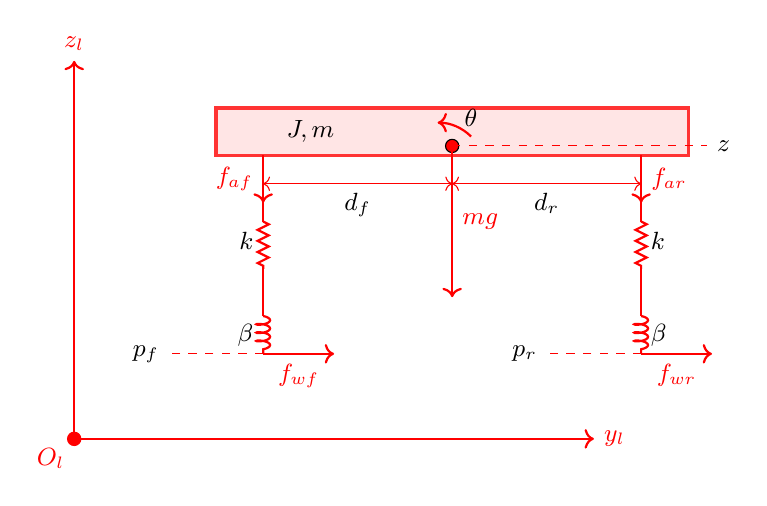
\begin{tikzpicture}[scale=1.2, every node/.style={font=\small}]
			
			% Coordinate axes
			\draw[->, thick, red] (-3.5,-1.5) -- (-3.5,2.5) node[above] {$z_l$};
			\draw[->, thick, red] (-3.5,-1.5) -- (2,-1.5) node[right] {$y_l$};
			\filldraw[red] (-3.5,-1.5) circle (2pt) node[below left] {$O_l$};
			
			% Sprung mass (body)
			\filldraw[color=red!80, fill=red!10, very thick] (-2,1.5) rectangle (3,2);
			\node at (-1,1.75) {$J, m$};
			
			% Center of mass
			\draw[fill=red] (0.5,1.6) circle (0.07);
			\draw[->, thick, red] (0.5,1.6) -- (0.5,0) node[midway,right] {$mg$};
			
			% pitch angle psi
			\draw[->, red, thick] (0,1.5) ++(0.7,0.2) arc[start angle=45,end angle=90,radius=0.5];
			\node at (0.7,1.9) {$\theta$};
			
			% Front suspension
			\draw[thick, red] (-1.5,1.5) -- (-1.5,0.8);
			\draw[thick, red, decorate, decoration={zigzag,segment length=4,amplitude=2}] (-1.5,0.8) -- (-1.5,0.3);
			\draw[thick, red] (-1.5,0.3) -- (-1.5,-0.2);
			\node[left] at (-1.5,0.6) {$k$};
			\draw[thick, red, decorate, decoration={coil,aspect=0.3, segment length=3}] (-1.5,-0.2) -- (-1.5,-0.6);
			\node[left] at (-1.5,-0.4) {$\beta$};
			\draw[->, thick, red] (-1.5,1.5) -- (-1.5,1.0) node[midway,left] {$f_{af}$};
			
			% Rear suspension
			\draw[thick, red] (2.5,1.5) -- (2.5,0.8);
			\draw[thick, red, decorate, decoration={zigzag,segment length=4,amplitude=2}] (2.5,0.8) -- (2.5,0.3);
			\draw[thick, red] (2.5,0.3) -- (2.5,-0.2);
			\node[right] at (2.5,0.6) {$k$};
			\draw[thick, red, decorate, decoration={coil,aspect=0.3, segment length=3}] (2.5,-0.2) -- (2.5,-0.6);
			\node[right] at (2.5,-0.4) {$\beta$};
			\draw[->, thick, red] (2.5,1.5) -- (2.5,1.0) node[midway,right] {$f_{ar}$};
			
			% Front and rear wheel forces
			\draw[->, thick, red] (-1.5,-0.6) -- (-0.75,-0.6) node[midway,below] {$f_{wf}$};
			\draw[->, thick, red] (2.5,-0.6) -- (3.25,-0.6) node[midway,below] {$f_{wr}$};
			
			% Ground heights
			\draw[dashed, red] (-1.5,-0.6) -- (-2.5,-0.6);
			\node[left] at (-2.5,-0.6) {$p_f$};
			\draw[dashed, red] (2.5,-0.6) -- (1.5,-0.6);
			\node[left] at (1.5,-0.6) {$p_r$};
			
			% Distances df and dr
			\draw[<->, red] (0.5,1.2) -- (-1.5,1.2);
			\node[below] at (-0.5,1.2) {$d_f$};
			\draw[<->, red] (0.5,1.2) -- (2.5,1.2);
			\node[below] at (1.5,1.2) {$d_r$};
			
			% Labels z
			\draw[dashed, red] (0.5,1.6) -- (3.2,1.6);
			\node[right] at (3.2,1.6) {$z$};
			
		\end{tikzpicture}
	\end{center}
	
	
%	
%	\begin{center}
%		
%		\begin{tikzpicture}[scale=1.2, every node/.style={font=\small}]
%			
%			% Coordinate axes
%			\draw[->, thick, red] (-3.5,-1.5) -- (-3.5,2.5) node[above] {$z_l$};
%			\draw[->, thick, red] (-3.5,-1.5) -- (2,-1.5) node[right] {$y_l$};
%			\filldraw[red] (-3.5,-1.5) circle (2pt) node[below left] {$O_l$};
%			
%			% Sprung mass (body)
%			\filldraw[color=red!80, fill=red!10, very thick] (-2,1.5) rectangle (3,2);
%			\node at (-1,1.75) {$J, m$};
%			
%			% Center of mass
%			\draw[fill=red] (0.5,1.6) circle (0.07);
%			\draw[->, thick, red] (0.5,1.6) -- (0.5,0) node[midway,right] {$mg$};
%			
%			% pitch angle theta
%			\draw[->, red, thick] (0,1.5) ++(0.7,0.2) arc[start angle=45,end angle=90,radius=0.5];
%			\node at (0.7,1.9) {$\theta$};
%			
%			% --- Front suspension ---
%			\draw[thick, red] (-1.5,1.5) -- (-1.5,0.8);
%			% Molla sospensione k
%			\draw[thick, red, decorate, decoration={zigzag,segment length=4,amplitude=2}] (-1.5,0.8) -- (-1.5,0.3);
%			\node[left] at (-1.5,0.6) {$k$};
%			\draw[thick, red] (-1.5,0.3) -- (-1.5,-0.1);
%			% Smorzatore beta
%			\draw[thick, red, decorate, decoration={coil,aspect=0.3, segment length=3}] (-1.5,-0.1) -- (-1.5,-0.5);
%			\node[left] at (-1.5,-0.3) {$\beta$};
%			\draw[thick, red] (-1.5,-0.5) -- (-1.5,-0.7);
%			% NUOVA: Molla pneumatico kt
%			\draw[thick, red, decorate, decoration={zigzag,segment length=4,amplitude=2}] (-1.5,-0.7) -- (-1.5,-1.2);
%			\node[left] at (-1.5,-0.95) {$k_t$};
%			\draw[thick, red] (-1.5,-1.2) -- (-1.5,-1.3);
%			
%			\draw[->, thick, red] (-1.5,1.5) -- (-1.5,1.0) node[midway,left] {$f_{af}$};
%			
%			% --- Rear suspension ---
%			\draw[thick, red] (2.5,1.5) -- (2.5,0.8);
%			% Molla sospensione k
%			\draw[thick, red, decorate, decoration={zigzag,segment length=4,amplitude=2}] (2.5,0.8) -- (2.5,0.3);
%			\node[right] at (2.5,0.6) {$k$};
%			\draw[thick, red] (2.5,0.3) -- (2.5,-0.1);
%			% Smorzatore beta
%			\draw[thick, red, decorate, decoration={coil,aspect=0.3, segment length=3}] (2.5,-0.1) -- (2.5,-0.5);
%			\node[right] at (2.5,-0.3) {$\beta$};
%			\draw[thick, red] (2.5,-0.5) -- (2.5,-0.7);
%			% NUOVA: Molla pneumatico kt
%			\draw[thick, red, decorate, decoration={zigzag,segment length=4,amplitude=2}] (2.5,-0.7) -- (2.5,-1.2);
%			\node[right] at (2.5,-0.95) {$k_t$};
%			\draw[thick, red] (2.5,-1.2) -- (2.5,-1.3);
%			
%			\draw[->, thick, red] (2.5,1.5) -- (2.5,1.0) node[midway,right] {$f_{ar}$};
%			
%			% Front and rear wheel forces (posizionate a fine kt)
%			\draw[->, thick, red] (-1.5,-1.3) -- (-0.75,-1.3) node[midway,below] {$f_{wf}$};
%			\draw[->, thick, red] (2.5,-1.3) -- (3.25,-1.3) node[midway,below] {$f_{wr}$};
%			
%			% Ground heights
%			\draw[dashed, red] (-1.5,-1.3) -- (-2.5,-1.3);
%			\node[left] at (-2.5,-1.3) {$p_f$};
%			\draw[dashed, red] (2.5,-1.3) -- (1.5,-1.3);
%			\node[left] at (1.5,-1.3) {$p_r$};
%			
%			% Distances df and dr
%			\draw[<->, red] (0.5,1.2) -- (-1.5,1.2);
%			\node[below] at (-0.5,1.2) {$d_f$};
%			\draw[<->, red] (0.5,1.2) -- (2.5,1.2);
%			\node[below] at (1.5,1.2) {$d_r$};
%			
%			% Labels z
%			\draw[dashed, red] (0.5,1.6) -- (3.2,1.6);
%			\node[right] at (3.2,1.6) {$z$};
%			
%		\end{tikzpicture}
		
		\begin{center}
	
		
		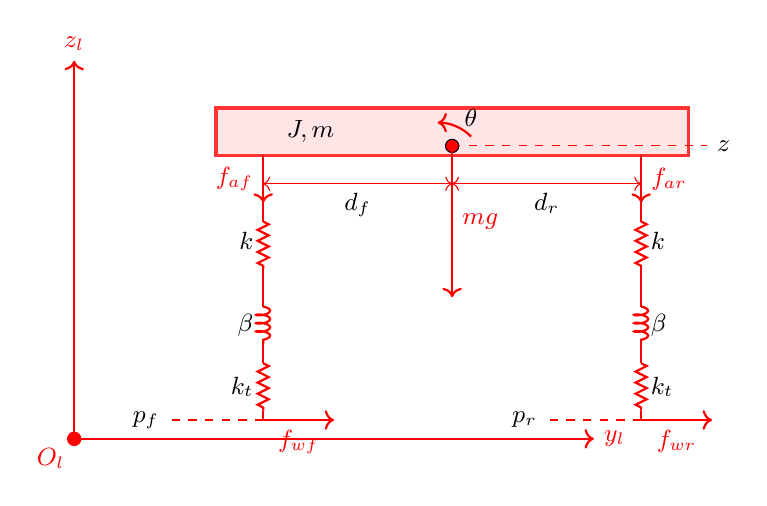
\begin{tikzpicture}[scale=1.2, every node/.style={font=\small}]
		
		% Coordinate axes
		\draw[->, thick, red] (-3.5,-1.5) -- (-3.5,2.5) node[above] {$z_l$};
		\draw[->, thick, red] (-3.5,-1.5) -- (2,-1.5) node[right] {$y_l$};
		\filldraw[red] (-3.5,-1.5) circle (2pt) node[below left] {$O_l$};
		
		% Sprung mass (body)
		\filldraw[color=red!80, fill=red!10, very thick] (-2,1.5) rectangle (3,2);
		\node at (-1,1.75) {$J, m$};
		
		% Center of mass
		\draw[fill=red] (0.5,1.6) circle (0.07);
		\draw[->, thick, red] (0.5,1.6) -- (0.5,0) node[midway,right] {$mg$};
		
		% pitch angle theta
		\draw[->, red, thick] (0,1.5) ++(0.7,0.2) arc[start angle=45,end angle=90,radius=0.5];
		\node at (0.7,1.9) {$\theta$};
		
		% --- Front suspension ---
		\draw[thick, red] (-1.5,1.5) -- (-1.5,0.8);
		% Molla sospensione k
		\draw[thick, red, decorate, decoration={zigzag,segment length=4,amplitude=2}] (-1.5,0.8) -- (-1.5,0.3);
		\node[left] at (-1.5,0.6) {$k$};
		\draw[thick, red] (-1.5,0.3) -- (-1.5,-0.1);
		% Smorzatore beta
		\draw[thick, red, decorate, decoration={coil,aspect=0.3, segment length=3}] (-1.5,-0.1) -- (-1.5,-0.5);
		\node[left] at (-1.5,-0.3) {$\beta$};
		\draw[thick, red] (-1.5,-0.5) -- (-1.5,-0.7);
		% NUOVA: Molla pneumatico kt
		\draw[thick, red, decorate, decoration={zigzag,segment length=4,amplitude=2}] (-1.5,-0.7) -- (-1.5,-1.2);
		\node[left] at (-1.5,-0.95) {$k_t$};
		\draw[thick, red] (-1.5,-1.2) -- (-1.5,-1.3);
		
		\draw[->, thick, red] (-1.5,1.5) -- (-1.5,1.0) node[midway,left] {$f_{af}$};
		
		% --- Rear suspension ---
		\draw[thick, red] (2.5,1.5) -- (2.5,0.8);
		% Molla sospensione k
		\draw[thick, red, decorate, decoration={zigzag,segment length=4,amplitude=2}] (2.5,0.8) -- (2.5,0.3);
		\node[right] at (2.5,0.6) {$k$};
		\draw[thick, red] (2.5,0.3) -- (2.5,-0.1);
		% Smorzatore beta
		\draw[thick, red, decorate, decoration={coil,aspect=0.3, segment length=3}] (2.5,-0.1) -- (2.5,-0.5);
		\node[right] at (2.5,-0.3) {$\beta$};
		\draw[thick, red] (2.5,-0.5) -- (2.5,-0.7);
		% NUOVA: Molla pneumatico kt
		\draw[thick, red, decorate, decoration={zigzag,segment length=4,amplitude=2}] (2.5,-0.7) -- (2.5,-1.2);
		\node[right] at (2.5,-0.95) {$k_t$};
		\draw[thick, red] (2.5,-1.2) -- (2.5,-1.3);
		
		\draw[->, thick, red] (2.5,1.5) -- (2.5,1.0) node[midway,right] {$f_{ar}$};
		
		% Front and rear wheel forces (posizionate a fine kt)
		\draw[->, thick, red] (-1.5,-1.3) -- (-0.75,-1.3) node[midway,below] {$f_{wf}$};
		\draw[->, thick, red] (2.5,-1.3) -- (3.25,-1.3) node[midway,below] {$f_{wr}$};
		
		% Ground heights
		\draw[dashed, red] (-1.5,-1.3) -- (-2.5,-1.3);
		\node[left] at (-2.5,-1.3) {$p_f$};
		\draw[dashed, red] (2.5,-1.3) -- (1.5,-1.3);
		\node[left] at (1.5,-1.3) {$p_r$};
		
		% Distances df and dr
		\draw[<->, red] (0.5,1.2) -- (-1.5,1.2);
		\node[below] at (-0.5,1.2) {$d_f$};
		\draw[<->, red] (0.5,1.2) -- (2.5,1.2);
		\node[below] at (1.5,1.2) {$d_r$};
		
		% Labels z
		\draw[dashed, red] (0.5,1.6) -- (3.2,1.6);
		\node[right] at (3.2,1.6) {$z$};
		
		\end{tikzpicture}
	\end{center}
	
	
	
	
	\textbf{todo: finire sto disegno}

	
	\begin{center} 
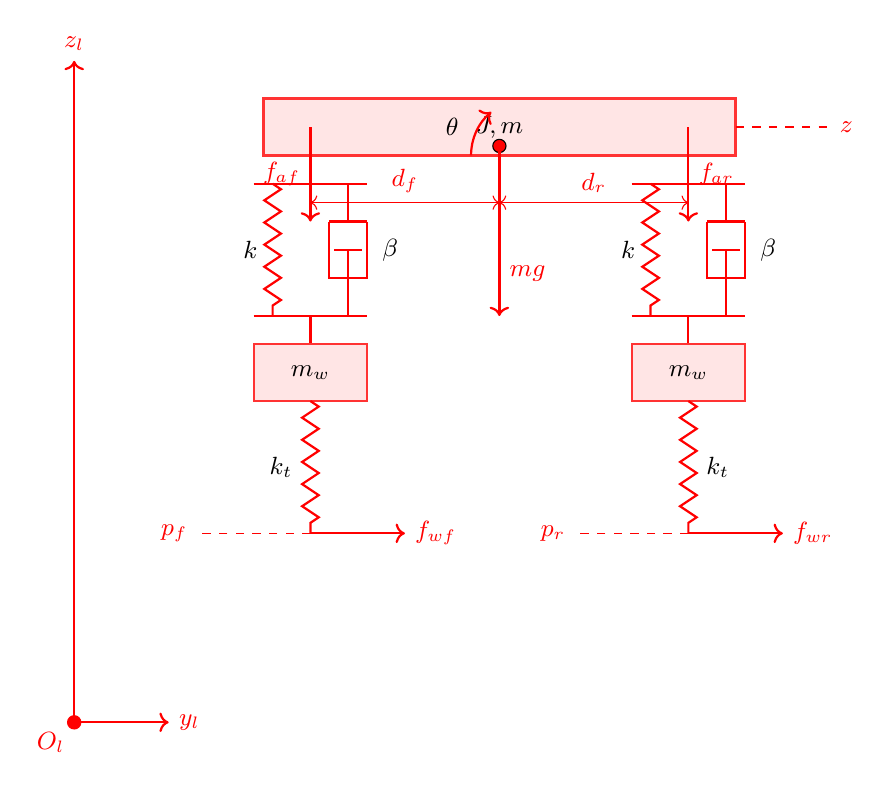
\begin{tikzpicture}[scale=1.2, every node/.style={font=\small}]
	% Coordinate axes - Spostati per non interferire
	\draw[->, thick, red] (-4,-3.5) -- (-4,3.5) node[above] {$z_l$};
	\draw[->, thick, red] (-4,-3.5) -- (-3,-3.5) node[right] {$y_l$};
	\filldraw[red] (-4,-3.5) circle (2pt) node[below left] {$O_l$};
	
	% --- SPRUNG MASS (Body) ---
	\filldraw[color=red!80, fill=red!10, very thick] (-2,2.5) rectangle (3,3.1);
	\node at (0.5,2.8) {$J, m$};
	
	% CM and Gravity
	\draw[fill=red] (0.5,2.6) circle (0.07);
	\draw[->, thick, red] (0.5,2.6) -- (0.5,0.8) node[right, near end] {$mg$};
	
	% Pitch angle theta
	\draw[->, red, thick] (0.2,2.5) arc[start angle=180, end angle=130, radius=0.6];
	\node at (0,2.8) {$\theta$};
	
	% --- FRONT SUSPENSION (Left) ---
	\def\xf{-1.5}
	% Connection to body
	\draw[thick, red] (\xf,2.5) -- (\xf,2.2);
	\draw[thick, red] (\xf-0.6,2.2) -- (\xf+0.6,2.2);
	
	% Sospensione superiore (k e beta parallelo) - DISTESA
	\draw[thick, red, decorate, decoration={zigzag,segment length=8,amplitude=3}] (\xf-0.4,2.2) -- (\xf-0.4,0.8);
	\node[left=2pt] at (\xf-0.4,1.5) {$k$};
	
	% Damper (beta)
	\draw[thick, red] (\xf+0.4,2.2) -- (\xf+0.4,1.8);
	\draw[thick, red] (\xf+0.2,1.8) -- (\xf+0.6,1.8); % Top cylinder
	\draw[thick, red] (\xf+0.2,1.8) -- (\xf+0.2,1.2) -- (\xf+0.6,1.2) -- (\xf+0.6,1.8); % Cylinder body
	\draw[thick, red] (\xf+0.25,1.5) -- (\xf+0.55,1.5); % Piston
	\draw[thick, red] (\xf+0.4,1.5) -- (\xf+0.4,0.8); % Rod
	\node[right=2pt] at (\xf+0.6,1.5) {$\beta$};
	
	\draw[thick, red] (\xf-0.6,0.8) -- (\xf+0.6,0.8);
	\draw[thick, red] (\xf,0.8) -- (\xf,0.5);
	
	% UNSPRUNG MASS (mw)
	\filldraw[color=red!80, fill=red!10, thick] (\xf-0.6,-0.1) rectangle (\xf+0.6,0.5);
	\node at (\xf, 0.2) {$m_w$};
	
	% TIRE STIFFNESS (kt) - DISTESA
	\draw[thick, red, decorate, decoration={zigzag,segment length=8,amplitude=3}] (\xf,-0.1) -- (\xf,-1.5);
	\node[left=3pt] at (\xf,-0.8) {$k_t$};
	
	% --- REAR SUSPENSION (Right) ---
	\def\xr{2.5}
	% Connection to body
	\draw[thick, red] (\xr,2.5) -- (\xr,2.2);
	\draw[thick, red] (\xr-0.6,2.2) -- (\xr+0.6,2.2);
	
	% Sospensione superiore (k e beta parallelo)
	\draw[thick, red, decorate, decoration={zigzag,segment length=8,amplitude=3}] (\xr-0.4,2.2) -- (\xr-0.4,0.8);
	\node[left=2pt] at (\xr-0.4,1.5) {$k$};
	
	% Damper (beta)
	\draw[thick, red] (\xr+0.4,2.2) -- (\xr+0.4,1.8);
	\draw[thick, red] (\xr+0.2,1.8) -- (\xr+0.6,1.8); 
	\draw[thick, red] (\xr+0.2,1.8) -- (\xr+0.2,1.2) -- (\xr+0.6,1.2) -- (\xr+0.6,1.8); 
	\draw[thick, red] (\xr+0.25,1.5) -- (\xr+0.55,1.5); 
	\draw[thick, red] (\xr+0.4,1.5) -- (\xr+0.4,0.8); 
	\node[right=2pt] at (\xr+0.6,1.5) {$\beta$};
	
	\draw[thick, red] (\xr-0.6,0.8) -- (\xr+0.6,0.8);
	\draw[thick, red] (\xr,0.8) -- (\xr,0.5);
	
	% UNSPRUNG MASS (mw)
	\filldraw[color=red!80, fill=red!10, thick] (\xr-0.6,-0.1) rectangle (\xr+0.6,0.5);
	\node at (\xr, 0.2) {$m_w$};
	
	% TIRE STIFFNESS (kt)
	\draw[thick, red, decorate, decoration={zigzag,segment length=8,amplitude=3}] (\xr,-0.1) -- (\xr,-1.5);
	\node[right=3pt] at (\xr,-0.8) {$k_t$};
	
	% --- FORCES AND GROUND ---
	% Ground forces
	\draw[->, thick, red] (\xf,-1.5) -- (\xf+1,-1.5) node[right] {$f_{wf}$};
	\draw[->, thick, red] (\xr,-1.5) -- (\xr+1,-1.5) node[right] {$f_{wr}$};
	
	% Ground inputs pf, pr
	\draw[dashed, red] (\xf,-1.5) -- (\xf-1.2,-1.5) node[left] {$p_f$};
	\draw[dashed, red] (\xr,-1.5) -- (\xr-1.2,-1.5) node[left] {$p_r$};
	
	% Distances df, dr
	\draw[<->, red] (0.5,2.0) -- (\xf,2.0) node[midway,above] {$d_f$};
	\draw[<->, red] (0.5,2.0) -- (\xr,2.0) node[midway,above] {$d_r$};
	
	% Active forces f_af, f_ar
	\draw[->, thick, red] (\xf,2.8) -- (\xf,1.8) node[midway,left] {$f_{af}$};
	\draw[->, thick, red] (\xr,2.8) -- (\xr,1.8) node[midway,right] {$f_{ar}$};
	
	% Reference height
	\draw[dashed, red] (3,2.8) -- (4,2.8) node[right] {$z$};
\end{tikzpicture}
	\end{center}
	Copy and past the Simulink block scheme and describe what each block does. Describe the set-up MATLAB file, where and how to change the parameters of the simulations. Remember to include also the sensor noises and realistic external disturbances.
	
	\section{Simulation results}
	Describe the simulation scenario: initial conditions, purpose of the simulation. Describe the results: are the results coherent with the expectation? If not why? Investigate the tuning: how the performance are affected by the selection of the parameters at disposal of the designer?
	
	\chapter{Conclusions and further investigation}
	Recap the main results obtained in the project and highlight eventual further investigation directions alogn which the performance could be improved. 
	
	\newpage
	\chapter*{Bibliography}
	List the papers/books cited.
	
	
	\newpage
	\appendix
	\chapter*{Appendix}
	Use appendices to add technical parts which are instrumental for the completeness of the manuscript but are too heavy to be included inside the main text. Basically, appendices are exploited to let the main text cleaner and smoother. As example, the complete MATLAB listings can be reported in appendix.\\
	
	
\end{document}          
